\section{Interpolation}
In this package, we have built various methods for interpolating a function; however, despite the simplicity of the method's implementation, a general analysis has been conducted on a specific method of implementing the function evaluation; this analysis will be presented after a brief description of the methods.

The following algorithm implementations that we have realized will be detailed in this section:
\begin{itemize}
    \item Polinomial Interpolation \algoref{alg:Polinomial Interpolation}
    \item Piecewise Linear Interpolation \algoref{alg:Piecewise Linear Interpolation}
    \item Piecewise Cubic Hermite Interpolation \algoref{alg:Piecewise Cubic Hermite Interpolation}
    \item Piecewise Cubic Interpolatory Splines \algoref{alg:Piecewise cubic Interpolatory Splines}
\end{itemize}

All this algorithms were based uppon Cleve's work~\cite{doi:10.1137/1.9780898717952}.
\subsection{Polynomial Interpolation}
This approach performs a polynomial interpolation of a given collection of points; it is one of the fundamental ways of interpolation and is widely taught in institutions.
\subsubsection{Examples}
	\paragraph{Example 1}{
\begin{lstlisting}[language=Python]
from BNumMet.Interpolation import polinomial
x = list(np.arange(1, 7, 1))
y = [16, 18, 21, 17, 15, 12]
u = np.arange(0.8, 6.2, 0.05)
v = polinomial(x, y, u)
# Plotting using Matplotlib
plt.plot(u, v, "b-", label="Interpolated")
plt.plot(x, y, "ro", label="Original Points")
plt.legend()
plt.show()
\end{lstlisting}
\begin{figure}[H]
    \centering
    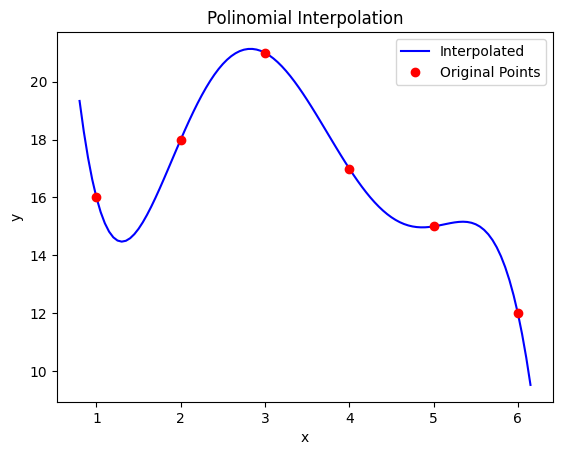
\includegraphics{Include/Images/Thesis/Documentation/Interpolation/Polinomial Example 1.png}
    \caption{Polinomial Linear Example 1}
    \label{fig:Polinomial Linear Example 1}
\end{figure}
}


\subsection{Piecewise linear interpolation}
Following the polynomial interpolation approach, the next step is to extend this notion to piecewise functions; in this manner, we accomplished the first step to utilizing a linear function.
\subsubsection{Examples}
	\paragraph{Example 1}{
\begin{lstlisting}[language=Python]
from BNumMet . Interpolation import piecewise_linear
x = list(np.arange(1, 7, 1))
y = [16, 18, 21, 17, 15, 12]
u = np.arange(0.8, 6.2, 0.05)
v = piecewise_linear(x, y, u)
# Plotting using Matplotlib
plt.plot(u, v, "b-", label="Interpolated")
plt.plot(x, y, "ro", label="Original Points")
plt.legend()
plt.show()
\end{lstlisting}
\begin{figure}[H]
    \centering
    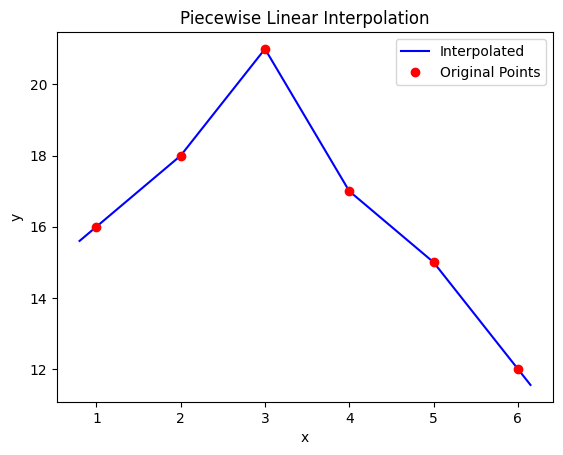
\includegraphics{Include/Images/Thesis/Documentation/Interpolation/PieceWise Linear Example 1.png}
    \caption{PieceWise Linear Example 1}
    \label{fig:PieceWise Linear Example 1}
\end{figure}
}

\subsection{Piecewise Cubic Hermite interpolation}
As a continuation of the previous method, we extended the concept of interpolating by Linear function to interpolating by a degree three polynomial with Hermite conditions, that is, by its values and first derivatives at the domain interval end points~\cite{kreyszig11}.
\subsubsection{Examples}
	\paragraph{Example 1}{
\begin{lstlisting}[language=Python]
from BNumMet.Interpolation import pchip
x = list(np.arange(1, 7, 1))
y = [16, 18, 21, 17, 15, 12]
u = np.arange(0.8, 6.2, 0.05)
v = pchip(x, y, u)
# Plotting using Matplotlib
plt.plot(u, v, "b-", label="Interpolated")
plt.plot(x, y, "ro", label="Original Points")
plt.legend()
plt.show()
\end{lstlisting}

\begin{figure}[H]
    \centering
    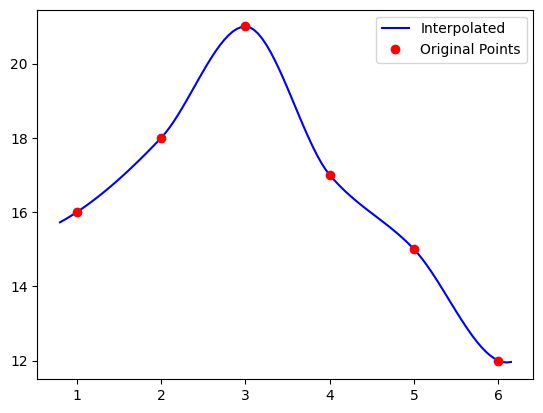
\includegraphics{Include/Images/Thesis/Documentation/Interpolation/PCHIP Example 1.png}
    \caption{PCHIP Example 1}
    \label{fig:PCHIP Example 1}
\end{figure}
}


\subsection{Piecewise cubic interpolation}
Following the Hermite interpolation, a more general approach in which we impose the slopes given by the not-a-knot end conditions, that is, at the first and last interior break, even the third derivative is continuous (up to round-off error) ~\cite{PCHIP}.

\subsubsection{Examples}
	\paragraph{Example 1}{
\begin{lstlisting}[language=Python]
from BNumMet.Interpolation import splines
x = list(np.arange(1, 7, 1))
y = [16, 18, 21, 17, 15, 12]
u = np.arange(0.8, 6.2, 0.05)
v = splines(x, y, u)
# Plotting using Matplotlib
plt.plot(u, v, "b-", label="Interpolated")
plt.plot(x, y, "ro", label="Original Points")
plt.legend()
plt.show()
\end{lstlisting}
\begin{figure}[H]
    \centering
    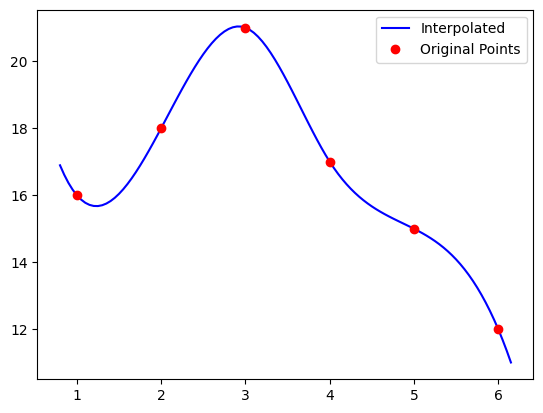
\includegraphics{Include/Images/Thesis/Documentation/Interpolation/Splines Example 1.png}
    \caption{Splines Example 1}
    \label{fig:Splines Example 1}
\end{figure}

}

\subsection{Interpolation implementation analysis}

Similar to the discussion in the linear systems package, we discovered various ways a student could implement one part of the method, specifically interpolation, by referring to the lines of code that calculate what value a point of the mesh (without the interpolation points) has as a y-coordinate. The code section may be summarized as follows: 



\begin{algorithm}[H]
\SetAlgoLined
\For{$j \gets 1$ \KwTo $n-2$} {
$k[x_j <= u] \gets j$
}
$s \gets u - x_k$\\
$v \gets y_k + s * \Delta_k$

\caption{Extract from Interpolation's algorithm}
\end{algorithm}
It should be noted that other algorithms may have different calculations, however for the sake of simplicity, we are generalizing the portion of code.


We might implement this section of code in a variety of ways, including:
\begin{enumerate}
    \item List Comprehension: Python offers a compact form for adding items to a list, in particular list comprehension, for a general reader a list comprehension is based on mathematical notation that is $\left\{ 3n\ |\ \forall n\in 0...25\right\}$ can be written in Python as \lstinline|[3*n for n in range(0,26)]|, generally speaking list comprehension is faster than classical loops~\cite{PythonSpeedPerformanceTips}, however, a better approach would be using functional maps which are cognitively more difficult to understand, thus not the purpose of this project.

    \item Using NumPy's \textit{fancy} Indexing: Similarly to Matlab, NumPy offers a way to broadcast a list, that is we can access the items of a list using another list, even though it is cognitively more complicated than list comprehensions; it is a syntax that is widely used in the numerical methods realm and might be a fair competitor over list comprehensions.
    
\end{enumerate}
\paragraph{Results}
To correctly test the implementations we will fix 6 interpolation pairs and then run 100 iterations for different meshes sizes with random values (to also check the ability to sort the mesh points), then after those 100 iterations are over, we will calculate the mean, the results are the following:
\begin{figure}[H]
    \centering
    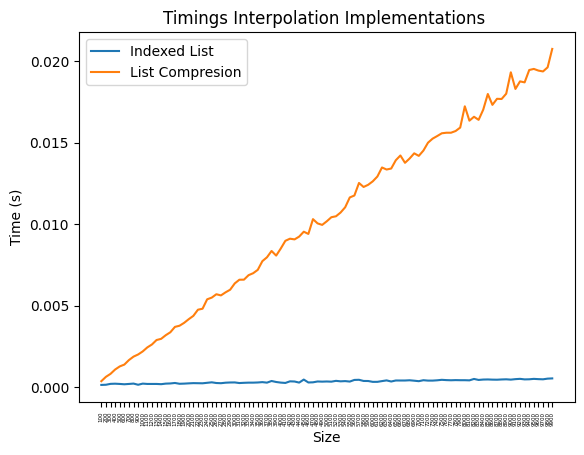
\includegraphics[scale=0.9]{Include/Images/Thesis/Analysis of Solutions/Interpolation/Interpolation Timings.png}
    \caption{Interpolation Timings}
    \label{fig:Interpolation Timings}
\end{figure}

As we can visually observe, the use of List Comprehensions is by far the worst of the two, and should be discarded for this particular case. We can also see how much the \textit{fancy} indexing improves the overall speed; that is why applying linear regression on the data, we have:
\begin{enumerate}
    \item \textbf{Linear Regression \textit{fancy} indexing}: \\
        $y = 3.4812\cdot10^{-08}x + 0.0002$ \\
        Slope: $3.48119\cdot10^{-08}$
    \item \textbf{Linear Regression List Compresion}: \\
        $y = 2.0237\cdot10^{-06}x + 0.0003$ \\
        Slope: $2.02374\cdot10^{-06}$
\end{enumerate}

Overall, not only does the choice of \textit{fancy} indexing is by far the fastest (around 2 orders of magnitude) but it also provides students a syntax that will be used during their learning of numerical methods, though it must be noted, the use of for-loops might be ideal for didactic purposes to teach students what could be behind the notation of this \textit{fancy} indexing.




